\documentclass{standalone}
% \documentclass{paper}
\usepackage{D:/DevData/LaTeX_Workplace/2_macro_definition/network_tikz_package}

\begin{document}

\begin{tikzpicture}
    \draw[help lines] (-3,-10) grid (10,10);
        % Use the new command to draw a single rounded rectangle
    % \rSquare{0.6}{NekasuBlue}{20}{5pt}{0}{0}{rs1}

    %表示图像中两个元素之间的水平偏移
    \def\offX{2.5}
    %表示图像中两个元素之间的垂直偏移
    \def\offY{3}
    % % 一个用于表示原始风格图像的node
    \coordinate (C) at (0,0);
    \node at (C) (C_fig) {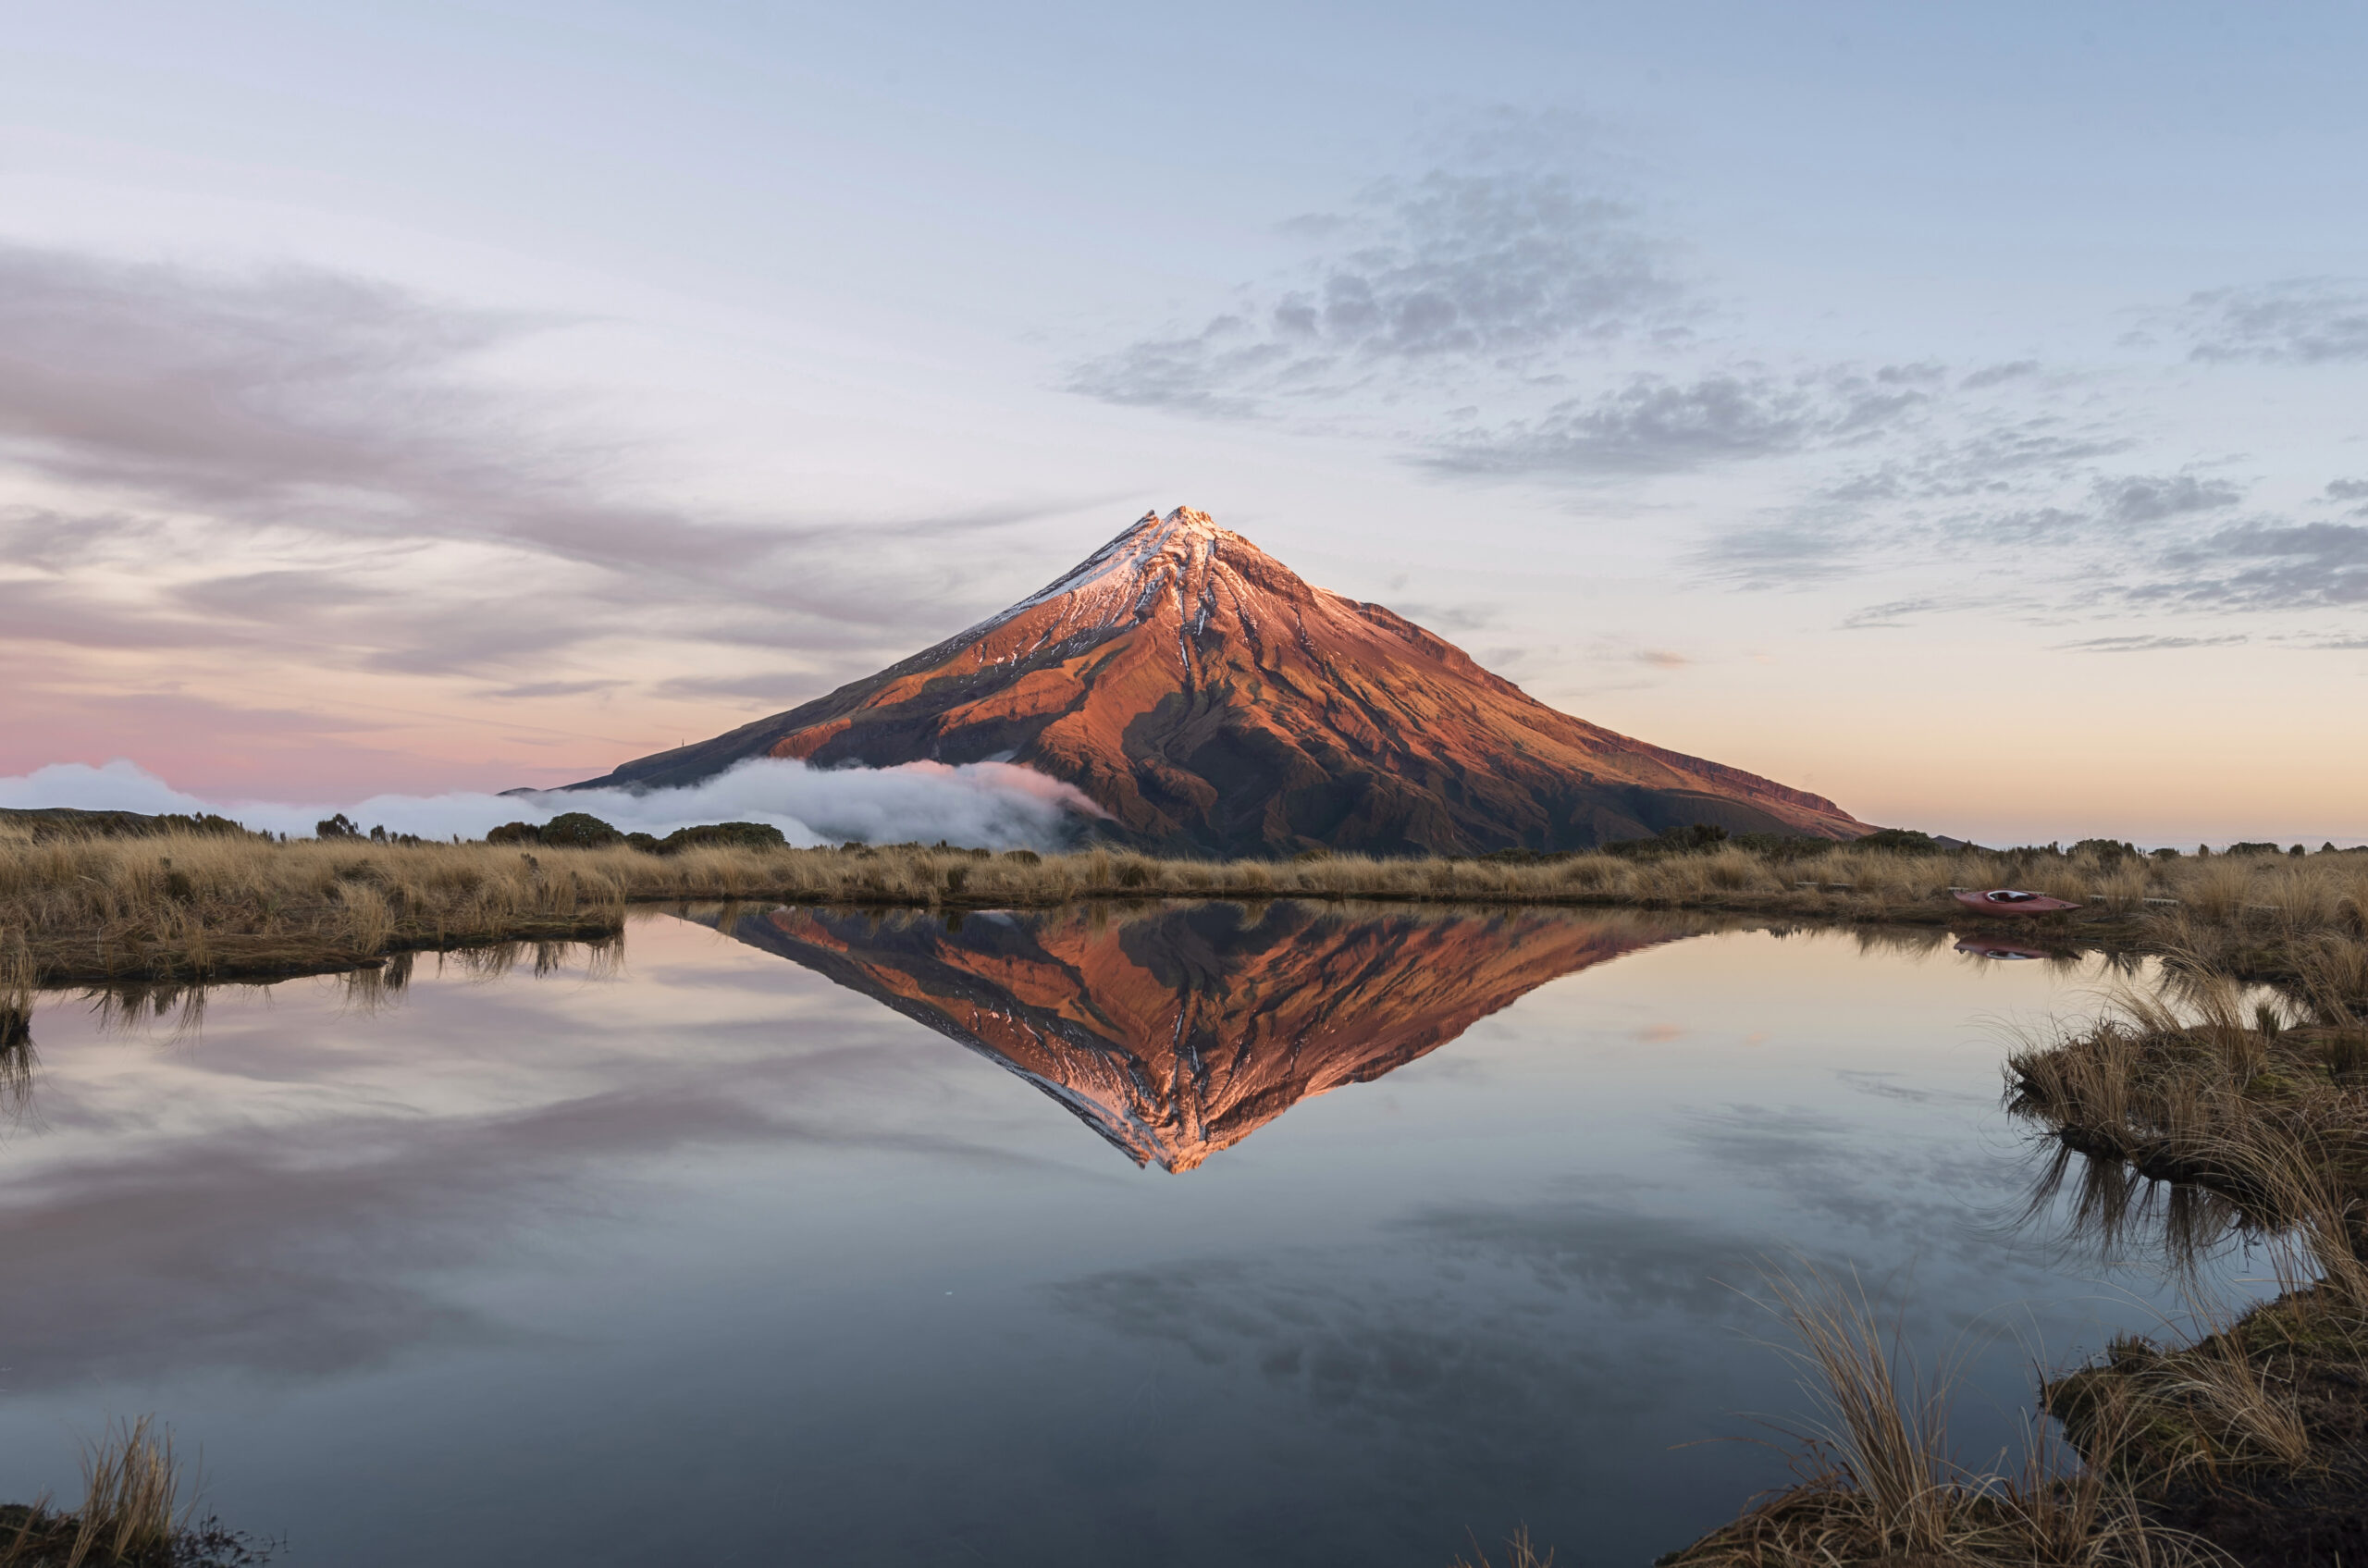
\includegraphics[width=2.5cm]{../pics/Content.jpeg}};
    % \node at ($(C)+(0,-1)$) (C_text) {$C$};
    

    %创建一个方形, 用于表示图像的高频部分H, 
    \coordinate (H) at ($(C)+(\offX+1,+1.5)$);
    \def\widthH{1.2};
    \coordinate (H_left_bottom) at ($(H)+(-\widthH/2,-\widthH/2)$);
    \coordinate (H_right_bottom) at ($(H)+(\widthH/2,\widthH/2)$);
    \coordinate (H_left) at ($(H)+(-\widthH/2-0.1,0)$);
    \coordinate (H_right) at ($(H)+(\widthH/2+0.1,0)$);
    \coordinate (H_upper) at ($(H)+(0,\widthH/2+0.1)$);
    \coordinate (H_bottom) at ($(H)+(0,-\widthH/2-0.1)$);
    \draw (H_left_bottom) rectangle (H_right_bottom);
    \node at ($(H)+(0,-\widthH/2-0.5)$) (H_text) {$H$};
    
    %创建一个方形, 用于表示图像的高频降噪部分Hdenoised
    \coordinate (Hdenoised) at ($(H)+(\offX,0)$);
    \def\widthHdenoised{1.2};
    \coordinate (Hdenoised_left_bottom) at ($(Hdenoised)+(-\widthHdenoised/2,-\widthHdenoised/2)$);
    \coordinate (Hdenoised_right_bottom) at ($(Hdenoised)+(\widthHdenoised/2,\widthHdenoised/2)$);
    \coordinate (Hdenoised_left) at ($(Hdenoised)+(-\widthHdenoised/2-0.1,0)$);
    \coordinate (Hdenoised_right) at ($(Hdenoised)+(\widthHdenoised/2+0.1,0)$);
    \coordinate (Hdenoised_upper) at ($(Hdenoised)+(0,\widthHdenoised/2+0.1)$);
    \coordinate (Hdenoised_bottom) at ($(Hdenoised)+(0,-\widthHdenoised/2-0.1)$);
    \draw (Hdenoised_left_bottom) rectangle (Hdenoised_right_bottom);
    \node at ($(Hdenoised)+(0,-\widthHdenoised/2-0.5)$) (Hdenoised_text) {$L$};

    %创建一个方形, 用于表示图像的高频部分L
    \coordinate (Low) at ($(C)+(\offX+1,-1.5)$);
    \def\widthLow{1.2};
    \coordinate (Low_left_bottom) at ($(Low)+(-\widthLow/2,-\widthLow/2)$);
    \coordinate (Low_right_bottom) at ($(Low)+(\widthLow/2,\widthLow/2)$);
    \coordinate (Low_left) at ($(Low)+(-\widthLow/2-0.1,0)$);
    \coordinate (Low_right) at ($(Low)+(\widthLow/2+0.1,0)$);
    \coordinate (Low_upper) at ($(Low)+(0,\widthLow/2+0.1)$);
    \coordinate (Low_bottom) at ($(Low)+(0,-\widthLow/2-0.1)$);
    \draw (Low_left_bottom) rectangle (Low_right_bottom);
    \node at ($(Low)+(0,-\widthLow/2-0.5)$) (Low_text) {$L$};
\end{tikzpicture}

\end{document}
